\chapter{Background}
\label{chap:bg}

In this chapter we introduce the concept of a masterserver and describe why legacy games depend on it.

\section{Finding a game}
The primary purpose that is to be accomplished, is to serve the paying customer, a choice in what game server he or she wants to join. Still as a business, the publisher's intended result is that a paying customer gets to play a game with other paying customers, who all involve others to buy the title and play too. The business model for this concept has changed significantly over the past two decades, but the focus is on the experience of the player.

Many games provide the option to play with or against other players. Usually there is a menu item called ``Multiplayer'' or ``Online Game'', that presents the player with a list of game servers that are currently online. A few clicks later, the player can shoot other players or conquer an evil enemy together. The focus in this document is in describing how the mechanics of acquiring this list work. To illustrate various functions and events, we use screenshots and examples from the game title ``Unreal Tournament'', as many of the games of that particular era are either based on or heavily influenced by this title.

\begin{figure}[h]
\centering
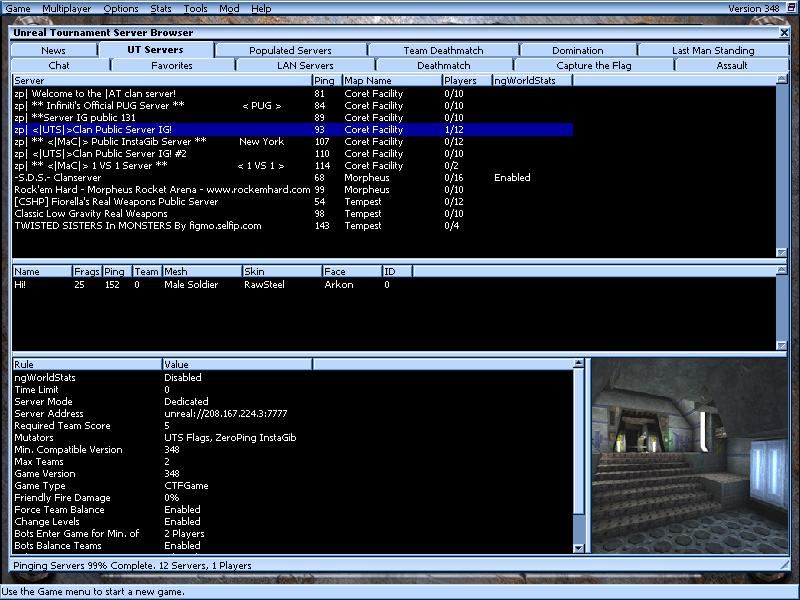
\includegraphics[width=0.7\textwidth]{./img/ubrowser}
\caption{The Unreal Tournament server browser with several online gameservers.}
\label{fig:ubrowser}
\end{figure}

When the player opens the multiplayer functionality, a list of online servers opens. We refer to this as the \emph{server browser}. Its main purpose is to provide the player with the available game servers and their individual properties, such as number of active players and current level or map. In figure \ref{fig:ubrowser} we see an example of such a server browser where we can identify three significant areas with information.

In the area on top, we see a list of online game servers with the name of the server, network response time (ping), name of the map and number of players. With this information, the player can decide to join their favourite server by name or just join any of the populated servers to play. The second segment displays a list of players and detailed information per player, like his/her score, ping, model (body shape) and textures (looks). With this list, the player can assess whether their friends are already playing and waiting for them, browse different servers and find anyone with whom they have played before or decide to join new people with the same interest in the game.

The last segment displays detailed server information, like the game type and playing style, team settings, server administrator details and a prominent server level screenshot. This segment provides a lot of detailed information that may be relevant to the more experienced players or people who are looking for a specific combination of mutators (game modifications). The combination of the information presented in these three segments drive the player to select a server of their choosing and join it.

\section{Online games}
The concept of online gaming and communication of this information over the internet may be a bit vague at this point. Everybody plays from their own computer and it is not always clear what interaction occurs at which side of the internet connection. In order to illustrate the different kinds of networking, we compare online games with their analogue variants: chess and poker. With chess, the two players could be playing on the same board or could be a large distance apart and communicate their moves by telephone: player one states he moves his rook from coordinates A3 to E3 and player two could respond by telling to move his pawn from C7 to C6. Both players are aware of the moves on the board and are playing the same game. 

With poker, it will be a lot more difficult to keep players appraised of the same game information without telling each other which cards they are holding. This requires of an independent party, the dealer. This dealer would communicate with each player individually which cards (s)he received from the deck and whether this person raises the pot. These analogue representations of multiplayer games can be described as peer-to-peer (chess) and server-client (poker) approaches. With a peer-to-peer game, players are directly connected to each other and are both aware of all aspects in the game. With a server-client game, each player has their unique response that the others are unaware of and only the server is capable of exchanging information between the others. 

From the poker analogy, we continue to multiple games. In the local bar, several groups of people are playing different rounds of poker on each table in different room. Every room has its own table, dealer and participants, independent from all other rooms and tables. In order to participate in a round of poker, you therefore only need to remember the address of the bar in order to gain access to all of the poker tables. Once you enter the bar, you ask the barkeep in which rooms the poker tables are located. The barkeep will tell you which rooms there are and you can look around the rooms to decide which table you want to join. The barkeep represents the masterserver, who keeps a list of all servers (rooms or poker tables) that are available. You do not need to maintain a record of the ever changing room/table list, instead one can just access the information directly from the barkeep.

\section{Game interactions}
To illustrate the more technical interactions between dealers, barkeep and player, we create three roles: {\bf gameserver}, {\bf masterserver}\footnote{We refer to \emph{gameservers} and \emph{masterservers} instead of \emph{game-} and \emph{master} servers. The latter is correct English, but the former improves readability and avoids confusion about what type of server we explicitly try to describe.} and {\bf client} in figure \ref{fig:totaloverview}. Everybody with an internet connection and a copy of the game could host their own gameserver. When a gameserver is initialised, it repeatedly sends a signal to the masterserver (1). We refer to these signals as \emph{heartbeats}, as the masterserver listens for these signals to determine if the gameserver is active, similar to how we listen for heartbeats in the human body to determine if somebody is still alive. 

Game clients make a request to the masterserver to obtain a list of all servers that sent heartbeats and the masterserver provides this list (2). The client then inquires at all of these gameservers for their information (or \emph{status}) so that the user can make a choice which gameserver to join (3).

\begin{figure}[ht]
\centering
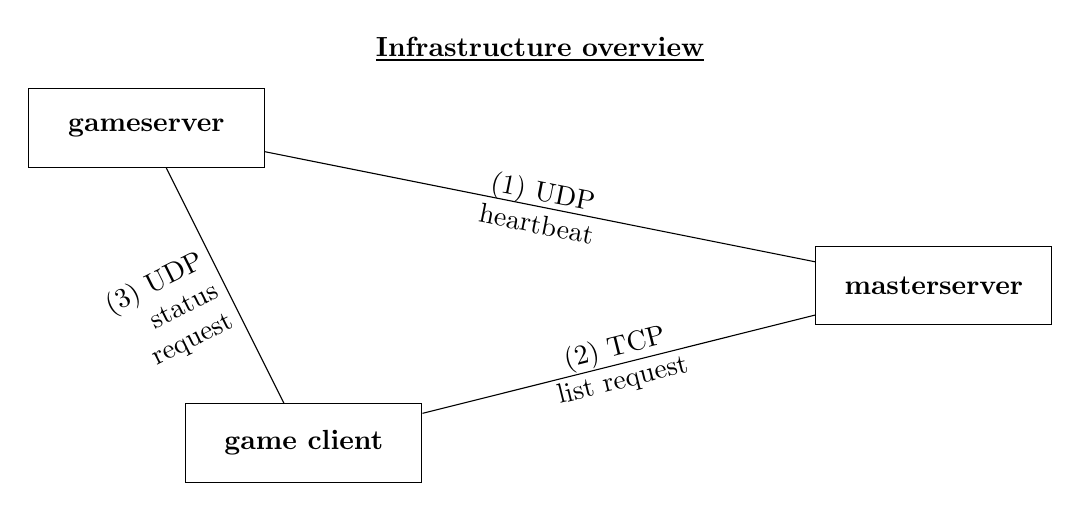
\begin{tikzpicture}

\tikzset{drawbox/.style={draw, rectangle, minimum height=1cm, minimum width=3cm}}
\tikzset{drawline/.style={midway, sloped, text width=2cm, text centered}}

% figure title
\node[rectangle] at (5, 1) (title) {\underline{\bf Infrastructure overview}};

% gameserver, masterserver, game client
\node[drawbox] at ( 0,  0) (gs) {\bf gameserver};
\node[drawbox] at (10, -2) (ms) {\bf masterserver};
\node[drawbox] at ( 2, -4) (gc) {\bf game client};

% interactions
\draw (gs) -- (ms) node[drawline] {(1) UDP\\heartbeat};
\draw (gc) -- (ms) node[drawline] {(2) TCP\\list request};
\draw (gc) -- (gs) node[drawline, rotate=90, left, align=right] {(3) UDP\\status request};


\end{tikzpicture}

\caption{General interactions between gameserver, masterserver and client.}\label{fig:totaloverview}
\end{figure}

All interactions between gameserver, masterserver and client occur over the internet. To avoid a wild growth of different methods to convey the information, GameSpy created a format of communication to handle many games with the same approach. When different gameservers follow the same protocol, the same interaction can be applied for a large variety in games. In other words, one barkeep could keep a room list for poker, monopoly, bridge and other games, instead of having one barkeep for every game: the masterserver can handle different games that use the same form of communication.

\section{Networking}
In the next chapters we address every interaction between gameserver, masterserver and client, but first we describe what we consider to be some required general knowledge about network communication and protocol. Since there is a variety of literature available for in-depth knowledge, we limit ourselves to the essential information that is necessary to understand the following chapters.\\

There are multiple methods to send information over the internet between peers. The two most important methods are \emph{UDP} and \emph{TCP} communication. Imagine that there is a speaker in front of a large audience. In order to get to know the audience, the speaker could ask everyone to shout their names. Everyone would shout their names one by one to the speaker and hope that the speaker would hear them properly. The \emph{user datagram protocol} (UDP) is similar to this situation: a gameserver sends a heartbeat to the masterserver, but there is no guarantee that information is correctly received or in the correct order.\\

The other method would be for the speaker to ask the audience to walk up to him one by one, shake hands and introduce themselves before sitting down again. The \emph{Transfer Control Protocol}  handles information in the same way: a client connects with the masterserver, identifies itself and retrieves the serverlist. As one could imagine, the information is conveyed correctly, but at the expense of a much larger duration of the interaction. The choice for either of these protocols in the game interactions is defined by the circumstances: some interactions require speed rather than precision, some interactions require precision over speed.

\section{Protocols}
Any form of communication, whether it is on the street, in the shop or digitally between two or more computers, follows a certain communication structure. During any meeting we often shake hands \footnote{This was before the global nCovid-19 pandemic.} and introduce ourselves before getting to business. This is called a \emph{protocol}. A protocol is a set of agreements that all communicating parties follow in order to convey information.

Many of the interactions that we discuss in this document follow the \emph{GameSpy} protocol. This protocol was, as the name suggests, developed by GameSpy Industries\cite{gs0} and contains a series of steps to perform the interactions as described in figure \ref{fig:totaloverview}. Many of the games published between 1995 and 2005 follow the GameSpy protocol and communicate in the same manner.

The GameSpy protocol formats the messages or data packets through backslashes. The general definition and examples of these messages are seen in example \ref{ls:gs0prot}, where the first line specifies the general format. The first word is a keyword, followed by a value, both prefixed by a backslash (line 1). Multiple keys and values can be appended to contain multiple game properties in a single message (line 2).

\lstinputlisting[caption={Example of the GameSpy protocol message formatting.}, stepnumber=1, label={ls:gs0prot}]{lst/gs0protocol.txt}

Digital data knows multiple data types, such as integers and floats for numbers, booleans for yes/no situations and strings for text. The GameSpy protocol has the versatility to transport all of these datatypes as plain text. Numbers can be conveyed as they are, either as integer (whole number) or float (decimal number) as seen in line 3. Boolean logic, like yes/no situations or 1/0 parameters are expressed through whole-word ``True'' or ``False'' values in line 4. Text is represented as-is and can contain spaces and special characters, as long as it is an ascii-character and not a backslash (line 5). 

The GameSpy protocol specifies a number of standardised key/value pairs that address the important functions in this infrastructure as we will be discussing in the next chapters. Over the years, there have been iterations and expansions of this protocol, as well as completely new and different protocols by different third parties. The 333networks masterserver that we describe in the following chapters uses the GameSpy protocol as foundation and expands from there where necessary.


